\documentclass{article}
\usepackage{graphicx}
\usepackage{pdfpages}
\usepackage{hyperref}
\usepackage[margin=1.25in]{geometry}

\hypersetup{
    colorlinks=true,
    linkcolor=blue,
    filecolor=magenta,      
    urlcolor=cyan,
}
\urlstyle{same}
\usepackage[font={small,it}]{caption}
\usepackage{fancyvrb}
\title{Analysis \& Visualization of Call Center Data using Python}
\author{John D. Bulger
\\
Karl Schmitt, Ph.D. (Advisor)
\\
Valparaiso University\\
}
\date{August 10, 2018}
\begin{document}
\maketitle

\begin{abstract}
\textit{The city of South Bend, Indiana operates a call center that serves as a primary point of contact for citizens.  The call center handles topics for nearly all of the city's departments.  An open data portal, maintained by the city, contains several years worth of information.  An analysis of this data was conducted using Python 3.6.  The data was 
analyzed for patterns by time of year, department, and topics with varying methods.  The cleaned, manipulated, and explored data was then developed into an 
interactive dashboard using the Bokeh library.  In doing so, an interactive HTML file will be distributed to the city, which can then be utilized, modified, and possibly connected 
directly to the data source.  Upon completetion, this analysis identified insights that could be actionable by the city.  July was found to be the most voluminous month, which was shown to be statistically signficant through the use of a two-sided t-test.  Additionally, the departments of Solid Waste and Water Works, along with many of their sub-topics, had some of the highest call volumes.  When calls were analyzed by duration, however, many lower volume topics were shown to take longer to resolve.}
\end{abstract}

\section{Introduction}
The city of South Bend, located in northern Indiana, established a citizen-accessible call center in February 2013.  It addresses almost every aspect of city-citizen interaction, including waste pick-up and removal, water billing and disconnections, 
and code enforcement.  By serving as a central hub for communication, the call center is able to consolidate a substantial amount of data regarding citizens as consumers.  This data is available on South Bend's open data portal at \href{https://data-southbend.opendata.arcgis.com}{https://data-southbend.opendata.arcgis.com}.

	\subsection{Prior Work}

The purpose of this research is to uncover trends and insights that may be of use to call center management.  Within the scope of this analysis, call duration can be seen as the ``efficiency" measure within this call center, particularly on a topical basis.  This metric is identified by Baraka et al. as one of the primary measures to assess call center success.\cite{baraka}  The authors identify other parameters, but analyzing this operation's success level was not within the scope of this paper.
\par
Call center and queueing analysis has been the focus of academic research for years.  Brown et al. provide an excellent overview of the Poisson distribution modeling customer arrivals, as well as the accompanying assumptions.  While arrival distribution is not analyzed in this paper, the authors' assumptions are, for the most part, assumed to be true in this analysis.  These center around the general assumption that the customers and operators are statistically identical and that they all act independently.\cite{brown}  Zhang, Hong, and Zhang also descibe the arrival process as a Poisson distribution, but discuss models which may be more accurate alternatives.\cite{zhang}  They maintain some of the main assumptions as Brown.  As a result, differences in time-dependent parameters, customer attitudes and preferences, and operator skill levels are treated as neglegible.
\par
Call centers are a prime opportunity to utilize simulation techniques.  In fact, according to Bapat and Pruitte, simulation is the preferred method to analyze and determine the effectiveness of a call center.\cite{bapat}  It allows for evaluation of metrics beyond what a basic analysis encompasses.  For example, the scheduling of call agents should be optimized against call duration and abandonment, as documented by Saltzman and Mehrota.\cite{saltzman}  This could be viewed as a logical next step for this project, with this work discovering the baseline knowedge necessary to construct such a model.




	\subsection{Goals \& Desired Results}

The goal of this analysis and visualization task is to, at its core, provide the city of South Bend useful and actionable knowledge about its call center.  Given the information-rich nature of this project, an interactive graphical dashboard was chosen as the primary means to communicate results.  The city was most curious about trends based on time, departments, and topics.  Therefore, this project had four major analytical foci:  month of year, day of the week, department, and topic.


\section{Data}

The data to be analyzed was acquired in three distinct files.
\par
\textbf{Daily Data --} contains a daily summary of the call center data from the years 2013-2015.  It is organized with 637 records indexed by date, with each record containing information such as the number of calls presented, average wait time, average number of calls in queue, and number of abandoned calls for that day.
\par
\textbf{Case Data --} contains 488,601 rows of individual call data from 2013 through 2015.  Calls were logged anonymously with data such as date, duration, topic, and department.  This data format went obsolete when the current call system was implemented.
\par
\textbf{Topic Data --} contains many of the same attributes as the case data, but it reflects the city's current use of knowledge base articles.  This systemizes the format for recording issues for each call, since each topic has a standardized name.  This ensures topics and departments match across the list, allowing for efficient and accurate analysis.
\par
The data was then inspected for missing data and reasonableness.  The daily data was missing no data points.  In the case data, less than 4\% of the 488,601 observations contained missing data.  These rows were missing a significant proportion of their respective attributes, and thus were dropped completely from the data.  The topic data, however, was missing almost 90\% of entries into an attribute used for open-format comments.  Since a substantial amount was missing and it was irrelevant to the analysis, this attribute was dropped completely.  This dataset was missing no other data.  Preprocessing and transformation was conducted immediately to transform the attributes into more useful types, such as date-time and numeric objects.

\section{Analytical Methods}

\textbf{Call volume by month --} was conducted using the daily data, which provides aggregate totals by day for a 2-year period. The relevant data was manipulated by taking the mean of the daily call volume for every record in each month.  As an exercise in thoroughness, these findings were subjected to a two-sided t-test for statistical significance.  For the purposes of this test, the null hypothesis stated that ``the two months have identical expected values."  For the null hypothesis to be disproved, a standard threshold p-value of 0.05 was used.
\par
\textbf{Call volume by day of the week --} was conducted from data contained in two files: daily data and topic data.  The first conveniently had an attribute consisting of an integer corresponding to a weekday.  The topic data included a date of call, but it did not have a direct day attribute.  This attributed was created with the same format as the daily data, and the calls corresponding to each date were counted.  The two dataframes were then concantenated, providing the total number of calls for each date.  Once grouped by weekday, this yielded a distribution of total calls for each day of the week over a five year period.  This data was also subjected to a t-test as monthly call volume was.
\par
\textbf{Calls volume and duration by department --} were analyzed using the topic data, as the data contained recent and complete information regarding departments.  One major impediment in this data was the format of call duration, which did not utilize a fixed-length field.  For example, duration for one record was in the form ``2:34" for two minutes, thirty-four seconds.  However, for longer calls it could be in the form ``1:15:56" for one hour, fifteen minutes, and fifty-six seconds.  While beneficial visually, this would not function for any analysis.  The duration was converted into seconds, and stored as a numeric data type.
\par
\textbf{Call volume and duration by topic --} were analyzed from the topic data as well.  Among this dataset, 426 unique call topics existed.  The data was then processed to show total call count and average call duration by topics.  Once completed, the data was able to be sorted by volume and duration, allowing for one dataset to serve the purposes of analysis of both duration and volume.


\section{Analysis}

\textbf{Call volume by month --} was analyzed using the daily data.  Months with the highest average daily call volumes were July, April, June, and May (in that order).  The results can be viewed in Figure 1.  March, interestingly, has the lowest average volume by a large margin.  This is especially intriguing since it is immediately prior to what can be seen as the ``busy season".  The heatmap in Figure 2 shows the resulting p-value from the t-test between each pair of months' distributions.  An interesting point that appears is that June's call volumes are not statistically different from those in April.  March, however, has a statistically lower daily average than every other month.
\par

\textbf{Call volume by day of the week --} incorporated over 588,000 calls into the results.  In order to most clearly see the results, a series of boxplots are shown in Figure 3.  Upon evaluation, call volume trends highest on Monday, then steadily decreases as the work week continues on.  The 311 service allows for voicemails to be left after hours, allowing operators to call customers back during business hours.  This could be a reason for the higher number of calls on Monday and Tuesday, since a weekend's worth of calls are presumably being dealt with.  A heatmap is shown in Figure 4, which emphasizes the statistically different mean for each pairing of weekdays (with the exception of Wednesday and Thursday).
\par

\textbf{Calls by department --} were analyzed by two measures:  average duration and total volume.  Departments such as Solid Waste and Water Works had the highest call volumes, while Code Enforcement and the Mayor's Office had the longest average durations.  Given this incongruency, it is not immediately clear where the call center's resources are being focused.  As a more direct approach to the measure of total call volume, the total departmental call times were calculated.  This can be visualized in Figure 4.
\par

\textbf{Calls by topic --} were also analyzed by duration and volume.  When ranked by average duration, many obscure topics rose to the extremes.  Of the top 20 topics with the shortest duration, 19 had a total number of calls of less than three.  When viewed as a percentage of the total 202,500 call dataset, these calls are such a small proportion that it would give little actionable insight to the city.  A similar, though less extreme, situation occurred when viewing topics with longest duration.  In light of this exploration, it was determined that the most important results for the city to see would include only topics that composed a significant proportion of total calls.  When ranking by duration, only topics with total volume above the first quartile of total call volume were included.  This yielded results that could be viewed as more relevant to management.  Topics with long durations seemed to be centralized around complaints and billing issues, and quick topics were mostly comprised of general information inquiries.  When analyzed in this manner, there is a 195 second difference between the longest and shortest topics.
\par
Topic volume was dominated by topics within many of the top departments identified earlier in Figure 1.  The top two highest volume topics, by a large margin, were ``Miscellaneous Trash Information" and ``Water Miscellaneous".  This is reflective of positions of Solid Waste and Water Works in the departmental analysis.  In order to allow the city to effectively visualize this tandem effect, topics within the some of the busiest departments were plotted in an interactive jitterplot, as seen in Figure 4.

\section{Discussion}

While the above analysis yielded clear results, the call center did not have any specific questions for which it was seeking answers.  Instead, this project was geared towards discovering trends, patterns, and insights; these were then provided to the city so that they could formulate specific questions based on the story that was told by this data.  In order to provide this to city managment, a visualization dashboard was chosn as the most effective medium.  The Bokeh package was used to create interactive visualizations, and allowed the final product to be packaged into a HTML file and sent to the call center management.  In all, the dashboard includes visualizations of:

\begin{itemize}
  \item{Pie chart of total call time by department}
  \item{Histogram of call volume by day of week, overlaid, with legend providing hide/show capabilities}
  \item{Bar chart of topics with longest average call duration}
  \item{Bar chart of topics with shortest average call duration}
  \item{Jitterplot of call volume by topic within top departments}
  \item{Bar chart of call volume by month}
\end{itemize}

These charts all utilize various implementation of Bokeh tools, such as HoverTool, BoxZoom, Pan, and checkbox interactivity.  By incorporating these interactions into the dashboard, the result is a more dynamic, engaging product that is simple to interact with for employees outside of the technical fields.  An image of the final dashboard can be found at the end of this paper, while a live link can be accessed at \href{http://jdbul33.github.io/CallCenterDashboard.html}{http://jdbul33.github.io/CallCenterDashboard.html}.


\section{Conclusions}

In summary, this analysis and presentation of data trends can be viewed as a successful high-level exploration.  Trends and points emerged from this analysis that will surely be of interest to call center management, while more insights can surely be found while interacting with the visualization dashboard.  For the city, this study should serve to identify areas of business interest within the context of these findings, which could then warrant further exploration with more specific questions.  For example, the city may want to see day-of-week trends for a specific topic, or they may seek to see how the number of calls queued relate to the number of calls abandoned.  These more specific questions would necessarily arise from a specific business need, which could perhaps be identified from this study.

	\subsection{Opportunities for Further Work}

Several paths for further work on this topic exist; however, the exact approach depends on the city's desires.  Currently, this data is being expanded into a model that will run as a simulation to determine the effectiveness of the call center.  This research provides much insight into distribution of topics and their average by each day of the week.  The data used in this analysis can also be explored from the angle of creating a simulation.  By simply obtaining a weekly operator schedule from the city, an effective simulation can be built to evaluate staffing levels, customer satisfaction, and many other call center metrics.
\par
Another possible approach would be to develop another dashboard, or perhaps modify the current one, to interact directly with the call center's data source.  This would allow a live, current view of trending topics and departments.  Such a tool could allow call center management to be agile and preemptive regarding emerging trends.



\begin{thebibliography}{5}

\bibitem{baraka}
Baraka, H., Baraka H. \& El-Gamily, I. (2013). Assessing call centers' success: A validation of the DeLone and Mclean model for information system. \textit{Egyptian Informatics Journal, 14}, 99-108.

\bibitem{brown}
Brown, L., Gans, N., Mandelbaum, A., Sakov, A., Shen, H., Zeltyn, S., \& Zhao, L. (2005). Statistical analysis of a telephone call center: a queueing-science perspective. \textit{Journal of the American Statistical Association, 100(469)}, 36-50.

\bibitem{zhang}
Xiaowei Zhang, L. Jeff Hong, \& Jiheng Zhang. (2014). Scaling and modeling of call center arrivals. \textit{In Proceedings of the 2014 Winter Simulation Conference (WSC '14)}. IEEE Press, Piscataway, NJ, USA, 476-485.

\bibitem{bapat}
Vivek Bapat \& Eddie B. Pruitte, Jr.. (1998). Using simulation in call centers. \textit{In Proceedings of the 30th conference on Winter simulation (WSC '98)}, D. J. Medeiros, Edward F. Watson, John S. Carson, and Mani S. Manivannan (Eds.). IEEE Computer Society Press, Los Alamitos, CA, USA, 1395-1400.

\bibitem{saltzman}
Robert Saltzman \& Vijay Mehrotra. (2007). Managing trade-offs in call center agent scheduling: methodology and case study. \textit{In Proceedings of the 2007 Summer Computer Simulation Conference (SCSC '07)}. Society for Computer Simulation International, San Diego, CA, USA, 643-651.

\end{thebibliography}
\newpage

\begin{figure}[p]
  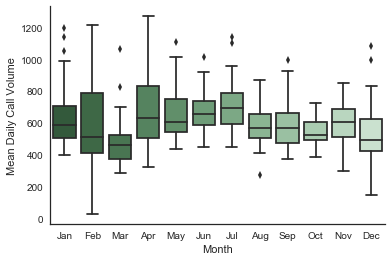
\includegraphics[scale=.6]{monthly_boxplot.png}
  \caption{Distribution of average daily call volume by month}
\end{figure}

\begin{figure}[p]
	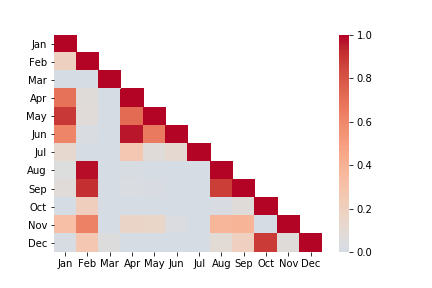
\includegraphics[scale=.5]{Heatmap.png}
	\caption{P-values resulting from t-test on daily call volume by month}
\end{figure}


\begin{figure}[p]
	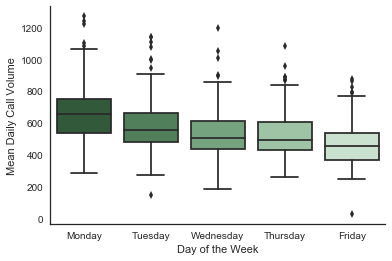
\includegraphics[scale=.6]{Daily_Call_Boxplot.png}
	\caption{Total daily calls by day of week}
\end{figure}

\begin{figure}[p]
	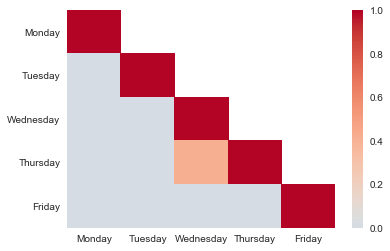
\includegraphics[scale=.5]{Daily_Heatmap.png}
	\caption{P-values resulting from t-test on daily call volume by day of the week}
\end{figure}

\begin{figure}[p]
	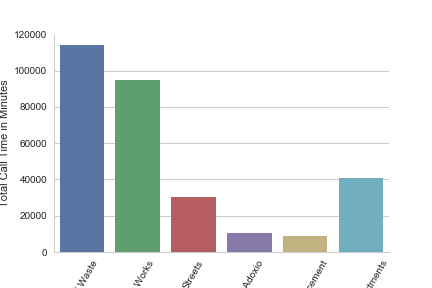
\includegraphics[scale=.6]{Calls_Department.png}
	\caption{Total Time Spent on Calls by Top Departments, 2016-2018}
\end{figure}

\begin{figure}[p]
  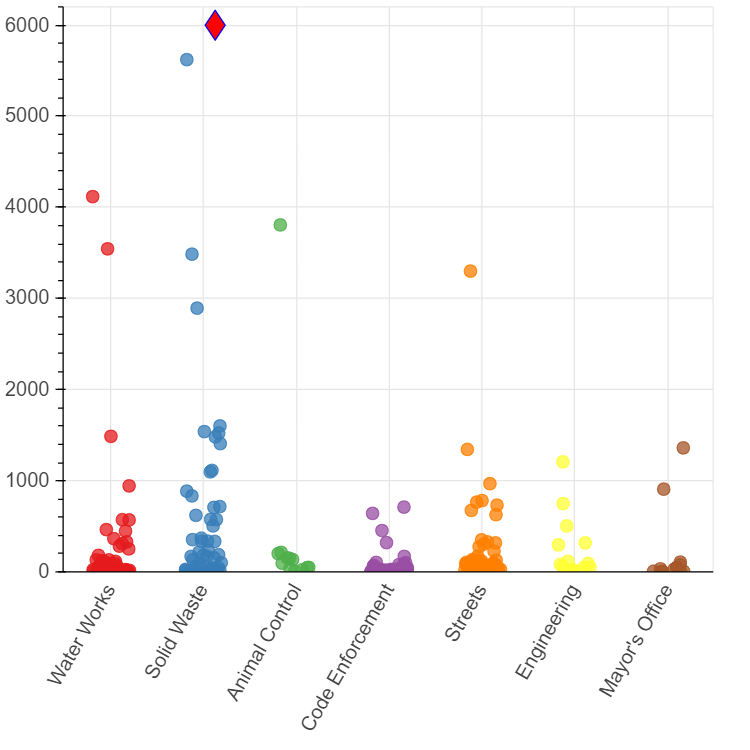
\includegraphics[scale=0.25]{jitterplot.png}
  \caption{Jitterplot of call volume by topic for the busiest departments.  Hovertool is utilized to show topic.  The topic in diamond is not plotted to scale}
\end{figure}

\end{document}

